\documentclass[twocolumn]{ltjsarticle}

\usepackage[top=20mm,bottom=20mm,left=20mm,right=20mm,columnsep=10mm]{geometry}
\usepackage[haranoaji,nfssonly]{luatexja-preset}
\usepackage{graphicx}
\usepackage{url}
\usepackage{multirow}  % セル結合用
\usepackage{tabularx}  % 表用&カラムサイズ指定

%% カラムサイズの指定用 %%
\newcolumntype{C}[1]{>{\centering\arraybackslash}p{#1}}
\newcolumntype{L}[1]{>{\raggedright\arraybackslash}p{#1}}
\newcolumntype{R}[1]{>{\raggedleft\arraybackslash}p{#1}}

\title{
  周期的な通信によるボットネット検出と対処優先度決定手法の提案  \\
  Detect and determine the risk level of botnets from periodic communication
}
\author{19FMI29 山下 尚彦 \and 研究指導教員 寺田 真敏}
\date{}

\begin{document}
\fontsize{9}{9}\selectfont
\maketitle

\section{はじめに}
パソコンやスマートフォン以外にも家電や自動車など多くのモノがインターネットに繋がるようになり,それらの機器(IoTデバイス)は2019年の時点で全世界で253億台,パソコンやスマートフォン,スマート家電などのコンシューマ向けのデバイスだけでも51億台もの端末がインターネットに接続されている\cite{総務省2020IoT:online}.サイバー攻撃の手法に,そのようなIoTデバイスを標的としたボットウイルスと呼ばれるマルウェアの一種に感染させて構築した巨大なネットワーク(ボットネット)を利用するものがあり,過去にはボットウイルスに感染した数百万台のデバイス(ボット)が接続されたボットネットが確認された.ボットネットによる攻撃はそのような巨大なネットワークを利用した手法が特徴で,そのひとつにボットネットに参加する複数の端末が攻撃命令を受けて外部のサーバに対して一斉にアクセスをしてサーバをダウンさせる分散型サービス拒否攻撃(Distributed Denial of Service attack,DDoS)攻撃がある.実際に2016年10月にDNSサービスを提供するアメリカの会社が,IoTデバイスを標的としたMiraiというボットウイルスによって構築されたボットネットからDDoS攻撃を受けた.その結果,一時的にサービスが停止し,そのサービスを利用していたTwitterやSpotify,PayPalなどの主要なサービスにも影響を受け,被害額が推定1億1000万ドルにもなった事件が起こった.また,DDoS攻撃以外にもスパムメールを配信する踏み台や仮想通貨を稼ぐためのマイニング,広告の自動クリックなど攻撃者の利益となる行為や脆弱なサーバ情報やクレジットカード番号の収集などのスパイウェアとしての活動にもボットネットは利用される.ボットウイルスは感染したデバイスに対して破壊活動や身代金の要求などを行わずに攻撃者の遠隔操作によって秘密裏に攻撃活動を行うため,ボットの発見は非常に困難である.

攻撃者はボットネットに接続する膨大な数のデバイスを制御するためにコマンド\&コントロール(C\&Cサーバ)と呼ばれる踏み台サーバを利用して攻撃命令や更新を行う.また,ボットネットに接続するデバイスに対して周期的に通信を行うことでボットネットが利用可能な状態か確認する.

本研究の目的はネットワークの通信を収集し,その周期性を分析することでC\&Cサーバとボットネットの周期的な通信の検出とC\&Cサーバからのレスポンスによって対処の優先度を決定する手法を提案する.

\section{関連研究}
本章では関連研究の概要と本研究との違いについて述べる.

AsSadhanらの研究\cite{assadhan2018analysis}ではボットネットとC\&Cサーバの通信によく用いられるプロトコルであるP2P,IRC,HTTPの既定のポート番号の11375,6667,80番ポート上の通信を収集し,周波数解析をすることでボットネットとC\&Cサーバ間の周期的な通信を検出する手法を提案した.実際に大学のネットワークで実験した結果,P2PとIRCによる通信の周期性を検出でき悪意のある通信を特定できたが,HTTPによる通信はボットウイルスの通信以外にも他のプログラムがHTTPを利用しているため膨大な通信量が発生したので検出が困難という結果となった.また,HTTPを利用したボットウイルスの検出が困難という問題の他に既定のポート番号で通信をフィルタリングしているため,独自のプロトコルを用いて通信を行うボットウイルスを検出できないとした.

本研究では通信の周期性を検出する際にポート番号で通信をフィルタリングするのではなく,送信元と受信先のIPアドレスごとに通信をグループに分けることによって他のプログラムの通信の影響を受けることなくボットウイルスの通信を検出可能とする.また,AsSadhanらの周波数解析で用いた手法とは違い,3.1.2項で説明するLomb-Scargleピリオドグラムによって不定間隔や欠損のある通信観測データであってもネットワークの通信の周期分析を行えるように変更する.

\section{提案手法}
本章ではボットネットとC\&Cサーバ間の周期的な通信からボットネットを検出する手法と対処の優先度を決定する手法を提案する.

\subsection{周期性のある通信の検出方法}
本節ではネットワークの通信を観測したデータ(通信観測データ)の前処理と周期性の検出,測定方法について述べる.

\subsubsection{解析前処理}
通信観測データから周期性の検出に必要な次の4つの情報を抽出する.
\begin{itemize}
  \item 通信時間のタイムスタンプ
  \item 送信元IPアドレス
  \item 受信先IPアドレス
  \item HTTPレスポンスステータスコード
\end{itemize}
通信時間のタイムスタンプと送信元IPアドレス,受信先IPアドレスは周期性の検出に,HTTPレスポンスステータスコードは対処優先度の決定に使用する.必要な情報を抽出後,送信元IPアドレスと受信先IPアドレスのペアとなるようにデータを加工する.

\subsubsection{周期性の検出}
本研究では3.1.1項で得られたデータをLomb-Scargleピリオドグラム\cite{vanderplas2018understanding}を用いて周波数解析することで通信の周期性を推定する.このLomb-Scargleピリオドグラムは不定間隔,または欠損のある信号であっても周波数を解析可能で,図\ref{fig:lombscargle}のような連続していない正弦波の周期性を推定できる.そのため,ネットワーク観測機器やソフトウェアの障害によって通信観測データが不完全な状態であっても周期的な通信の検出が期待できる.
\begin{figure}[htbp]
  \centering
  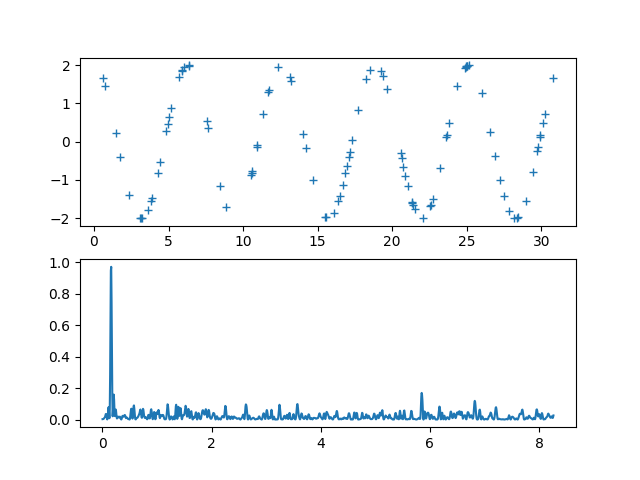
\includegraphics[width=8cm]{images/20201214_修士論文予稿/lombscargle.png}
  \caption{欠損のある正弦波と解析結果}
  \label{fig:lombscargle}
\end{figure}

\subsubsection{周期性の測定}
Lomb-Scargleピリオドグラムによる信号の周期性は,信号が周期性のない正規分布であると仮定して解析した結果,グラフのピークがしきい値を超えたかどうかで判断することができる.図\ref{fig:lombscargle}上部の正弦波に99\%周期性があるか測定する場合,正弦波が1\%の確率で非周期的であると仮定し,Lomb-Scargleピリオドグラムで周波数解析した結果である図\ref{fig:lombscargle}下部のグラフのピーク(=0.9993959064009751)が,この正弦波が99\%周期的であることを示す値(=0.18631798)を超えているため,図\ref{fig:lombscargle}の正弦波は99\%以上周期的であるといえる.

\subsection{対処優先度の決定}
HTTPプロトコルで通信したとき,レスポンスにリクエストが正常に完了したかを表す3桁の数字からなるHTTPレスポンスステータスコード(以下ステータスコード)が返送される.ステータスコードは主に,リクエストが正常に完了したことを表す200番台,URLの間違いによってサーバのリソースが発見できなかった404(Not Found)などのリクエスト側のエラーを表す400番台,サーバで処理できない事態が発生した500(Internal Server Error)などのレスポンス側で起きるエラーを表す500番台の数字が使われる.

本研究ではボットウイルスがC\&Cサーバから受け取るステータスコードに着目して対処の優先度を決定する.3.1節で示した方法で検出した周期性のある通信のうち,C\&Cサーバと正常に通信を行えていることを表す200番台のステータスコードを受け取った場合早急に対処する必要がある事案とし,400番台や500番台であったらリクエストが正常にできていないため対処の優先度を低くする.また,リクエストが正常にできていない場合でも,ステータスコードが400番台のときはC\&Cサーバは稼働しているがリクエスト側のエラーによって通信が行えていない可能性があるため,500番台よりも優先度を高く設定する.

\section{実験}
本章ではデータセットBOS\_2016の概要とデータセットに含まれているマルウェア検体の挙動や通信,実験に使用したデータや条件について述べる.

\subsection{BOS\_2016について}
本研究で使用するデータセットBOS\_2016は,総務省実証事業「サイバー攻撃解析・防御モデル実践演習の実証実験の請負」にて実施され,研究者コミュニティから提供された組織内ネットワークへの侵害活動を観測したデータセット\cite{マルウェア対策研42:online}である.BOS\_2016にはマルウェア検体のハッシュ値情報や通信観測データ,プロセス観測データ,Windowsのイベントログ,ファイアウォールのログデータがデータセットとして提供されている.

表\ref{tab:bos2016}は,寺田らがBOS\_2016について報告した論文\cite{weko_175829_1}を参考にマルウェア検体の挙動とC\&Cサーバとの通信についてまとめたものである.BOS\_2016にはマルウェア検体を実行できたもの(Case e04,e12,e20,e70,e435)と実行できなかったもの(Case e43)がある.また,マルウェア検体が動作した中でC\&Cサーバと正常に通信ができたのはe04のみで,それ以外の検体はボットウイルスやC\&Cサーバでエラーが発生したり,e70やe435のようにSYNパケットをC\&Cサーバに送信するがサーバから応答がないためそもそもTCPコネクションを確立できなかったりしたため,C\&Cサーバと正常に通信できなかった.
\begin{table}[htbp]
  \centering
  \caption{BOS\_2016の検体の挙動と通信について}
  \begin{tabular}{C{20mm}L{15mm}L{30mm}}
    %% カラム名 %%
    \hline
    Case & 挙動 & 通信 \\
    \hline \hline
    %% データ %%
    e04 & 動作 & 攻撃活動を観測 \\ \hline
    e12\par e20 & 動作 & C2サーバとの通信が成立しない(403, 404, 503) \\ \hline
    e43 & 実行不可 & 通信発生せず \\ \hline
    e70\par e435 & 動作 & C2サーバへSYNパケットのみ送信 \\
    \hline
  \end{tabular}
  \label{tab:bos2016}
\end{table}

\subsection{使用データと実験条件}
実験ではネットワークから周期性のある通信を検出するためにデータセットBOS\_2016でe43以外のマルウェア検体が動作した事例の通信観測データを使用する.また,e04はマルウェアが動作し攻撃活動を観測したため通信観測データが提供されていなかったため,e12からe435の通信観測データを用いてLomb-Scargleピリオドグラムによってネットワーク内の通信のうち99.9\%以上の確率で周期的な通信を行ったIPアドレスのペアを検出する.

\section{結果}
本章ではデータセットBOS\_2016の通信観測データをLomb-Scargleピリオドグラムで周波数解析した結果から周期性のある通信とステータスコードについて述べる.

\subsection{Case e12}
Case e12はC\&CサーバとTCPコネクションを確立できたがC\&Cサーバからのレスポンスステータスコードが403(Forbidden)や404(Not Found),503(Server Unavailable)などで通信が成立しなかった事例である.

表\ref{tab:e12_ip}はLomb-Scargleピリオドグラムによって周波数解析をした結果,マルウェア検体が99.9\%の確率で周期的な通信を行った通信先のIPアドレスである.e12のマルウェア検体のC\&CサーバのIPアドレスは\ast\ast\ast.56.81.119と\ast\ast\ast.76.86.155の2つで,実験の結果2016年2月12日にどちらも検出することができた事がわかる.
\begin{table}[htbp]
  \centering
  \caption{e12で周期的な通信を示した受信先IPアドレス}
  \begin{tabular}{|c||c|l|}
    \hline
    DATE & PERIODIC & IP ADDRESS \\
    \hline \hline
    2016/02/12 & 99.9\% & \begin{tabular}{l}
                            \textbf{\ast\ast\ast.56.81.119} \\
                            \textbf{\ast\ast\ast.76.86.155} \\
                            \ast\ast\ast.79.197.250         \\
                            \ast\ast\ast.32.241.24          \\
                          \end{tabular} \\ \hline
    2016/02/15 & 99.9\% & \begin{tabular}{l}
                            \ast\ast\ast.76.4.147   \\
                            \ast\ast\ast.59.139.27  \\
                            \ast\ast\ast.59.160.60  \\
                            \ast\ast\ast.213.168.19 \\
                          \end{tabular} \\ \hline
  \end{tabular}
  \label{tab:e12_ip}
\end{table}

図\ref{fig:e12_result1}と図\ref{fig:e12_result2}はそれぞれ,上部が2016年2月12日にマルウェア検体がC\&Cサーバ\ast\ast\ast.56.81.119と\ast\ast\ast.76.86.155と行った通信回数と通信発生時間に関するグラフで,下部がLomb-Scargleピリオドグラムで解析した結果である.図\ref{fig:e12_result1}上部からマルウェア検体がC\&Cサーバ\ast\ast\ast.56.81.119と通信した回数は186回で,解析結果のグラフからピークが0.5708873577625633ということがわかる.この通信が99.9\%周期的と判断できる値は0.1229852684658255のため,マルウェア検体とC\&Cサーバ\ast\ast\ast.56.81.119の通信は周期的であると言える.同様に,マルウェア検体がC\&Cサーバ\ast\ast\ast.76.86.155と通信した回数は40回,解析結果のピークが0.8867795437401563で99.9\%周期的と判断できる値は0.28275941645939073のため,マルウェア検体とC\&Cサーバ\ast\ast\ast.76.86.155の通信は周期的であると言える.
\begin{figure}[htbp]
  \centering
  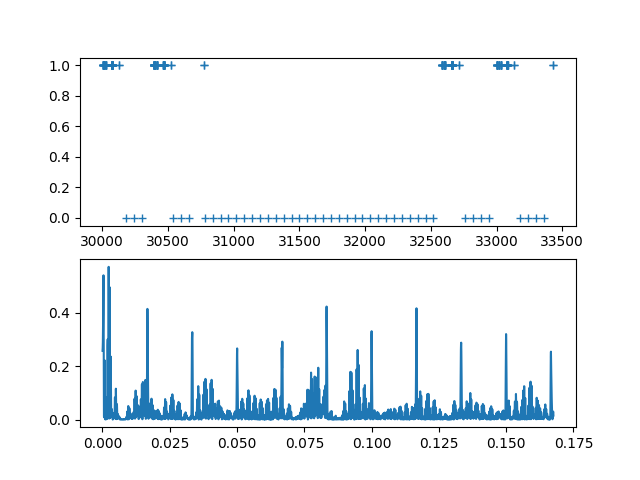
\includegraphics[width=8cm]{images/20201214_修士論文予稿/e12_c2_1.png}
  \caption{\ast\ast\ast.56.81.119の通信回数と解析結果}
  \label{fig:e12_result1}
\end{figure}
\begin{figure}[htbp]
  \centering
  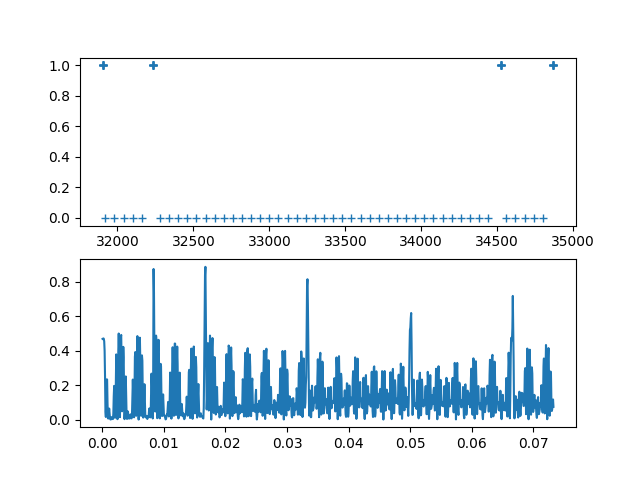
\includegraphics[width=8cm]{images/20201214_修士論文予稿/e12_c2_2.png}
  \caption{\ast\ast\ast.76.86.155の通信回数と解析結果}
  \label{fig:e12_result2}
\end{figure}

表\ref{tab:e12_status_code}はそれぞれのC\&Cサーバから返ってきたステータスコードの種類と回数の関係を表した表である.
\begin{table}[htbp]
  \centering
  \caption{ステータスコードの種類と回数}
  \begin{tabular}{|l||c|c|}
    \hline
    IP ADDRESS & 200(OK) & 403(Forbidden) \\
    \hline \hline
    \ast\ast\ast.56.81.119 & 4 & 16 \\ \hline
    \ast\ast\ast.76.86.155 & 4 & 3  \\ \hline
  \end{tabular}
  \label{tab:e12_status_code}
\end{table}

\subsection{Case e20}
Case e20はCase e12と同様に,C\&CサーバとTCPコネクションを確立できたが通信が成立しなかった事例である.

表\ref{tab:e20_ip}はe20のマルウェア検体が99.9\%の確率で周期的な通信を行った通信先のIPアドレスの一覧である.このマルウェア検体のC\&CサーバのIPアドレスは\ast\ast\ast.81.81.137である.しかし,表\ref{tab:e20_ip}から分かるように今回の実験ではマルウェア検体とC\&Cサーバ間の周期的な通信を検出できなかった.
\begin{table}[htbp]
  \centering
  \caption{e20で周期的な通信を示した受信先IPアドレス}
  \begin{tabular}{|c||c|l|}
    \hline
    DATE & PERIODIC & IP ADDRESS \\
    \hline \hline
    2016/02/15 & 99.9\% & \begin{tabular}{l}
                          \ast\ast\ast.32.1.160   \\
                          \ast\ast\ast.107.4.50   \\
                          \ast\ast\ast.58.221.163 \\
                        \end{tabular} \\ \hline
    2016/02/16 & 99.9\% & \begin{tabular}{l}
                          \ast\ast\ast.118.6.83
                        \end{tabular} \\ \hline
    2016/02/18 & 99.9\% & \begin{tabular}{l}
                          \ast\ast\ast.32.1.160    \\
                          \ast\ast\ast.36.102.106  \\
                          \ast\ast\ast.113.237.189 \\
                        \end{tabular} \\ \hline
  \end{tabular}
  \label{tab:e20_ip}
\end{table}

図\ref{fig:e20_count}はe20のマルウェア検体が行ったC\&Cサーバとの通信時間と通信回数の関係を表した図で,通信は1秒間に3回しか行われていないことが分かる.
\begin{figure}[htbp]
  \centering
  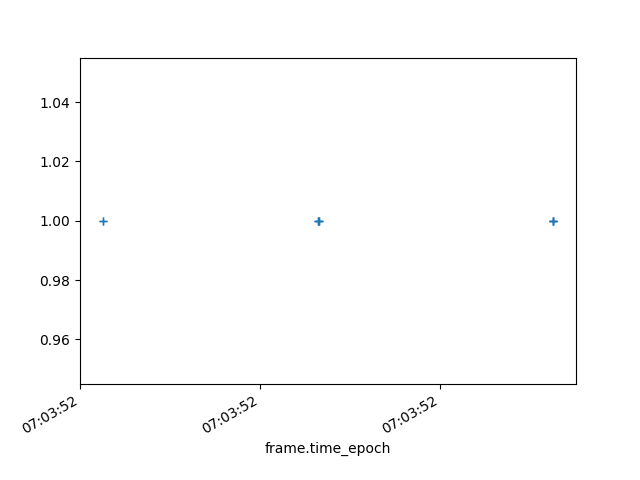
\includegraphics[width=8cm]{images/20201214_修士論文予稿/e20_count.png}
  \caption{\ast\ast\ast.81.81.137の通信回数}
  \label{fig:e20_count}
\end{figure}

C\&Cサーバとの通信を検出することができなかったため,ステータスコードも取得できなかった.

\subsection{Case e70}
Case e70はマルウェアが正常に動作したがC\&CサーバにSYNパケットを送信するのみでC\&Cサーバから返送がなくTCPコネクションを確立できなかった事例である.e70のマルウェア検体のC\&CサーバのIPアドレスは\ast\ast\ast.106.20.192である.

表\ref{tab:e70_ip}はマルウェア検体が99.9\%の確率で周期的な通信を行った通信先のIPアドレスの一覧である.表から2016年2月の15日から18日の4日間でC\&CサーバのIPアドレスを検出できた.
\begin{table}[htbp]
  \centering
  \caption{e70で周期的な通信を示した受信先IPアドレス}
  \begin{tabular}{|c||c|l|}
      \hline
      DATE & PERIODIC & IP ADDRESS \\
      \hline \hline
      2016/02/15 & 99.9\% & \begin{tabular}{l}
                            \textbf{\ast\ast\ast.106.20.192} \\
                            \ast\ast\ast.32.101.160          \\
                            \ast\ast\ast.165.83.176          \\
                            \ast\ast\ast.21.181.152          \\
                            \ast\ast\ast.208.153.9           \\
                            \ast\ast\ast.106.149.145         \\
                            \ast\ast\ast.106.253.18          \\
                          \end{tabular} \\ \hline
      2016/02/16 & 99.9\% & \begin{tabular}{l}
                            \textbf{\ast\ast\ast.106.20.192} \\
                            \ast\ast\ast.32.101.160          \\
                            \ast\ast\ast.165.83.176          \\
                            \ast\ast\ast.21.181.152          \\
                            \ast\ast\ast.208.153.9           \\
                            \ast\ast\ast.106.149.145         \\
                            \ast\ast\ast.106.253.18          \\
                          \end{tabular} \\ \hline
      2016/02/17 & 99.9\% & \begin{tabular}{l}
                            \textbf{\ast\ast\ast.106.20.192} \\
                            \ast\ast\ast.32.101.160          \\
                            \ast\ast\ast.165.83.176          \\
                            \ast\ast\ast.21.181.152          \\
                            \ast\ast\ast.208.153.9           \\
                            \ast\ast\ast.106.149.145         \\
                            \ast\ast\ast.106.253.18          \\
                          \end{tabular} \\ \hline
      2016/02/18 & 99.9\% & \begin{tabular}{l}
                            \textbf{\ast\ast\ast.106.20.192} \\
                            \ast\ast\ast.32.101.160          \\
                            \ast\ast\ast.165.83.176          \\
                            \ast\ast\ast.21.181.152          \\
                            \ast\ast\ast.208.153.9           \\
                            \ast\ast\ast.106.149.145         \\
                            \ast\ast\ast.106.253.18          \\
                          \end{tabular} \\ \hline
  \end{tabular}
  \label{tab:e70_ip}
\end{table}

図\ref{fig:e70_result}は2016年2月15日にe70のマルウェア検体とC\&Cサーバ間の通信時間と通信回数の関係を表した図である.通信が発生した時間は15分間で,合計1520回通信を行ったことが分かる.また,Lomb-Scargleピリオドグラムによる解析結果のグラフのピークは0.30098694754202543で99.9\%周期的と判断できる値の0.01843714305868322を超えているためマルウェア検体とC\&Cサーバの通信は周期的であると言える.C\&Cサーバとの通信を確認できた別日でも同様の結果を得られた.
\begin{figure}[htbp]
  \centering
  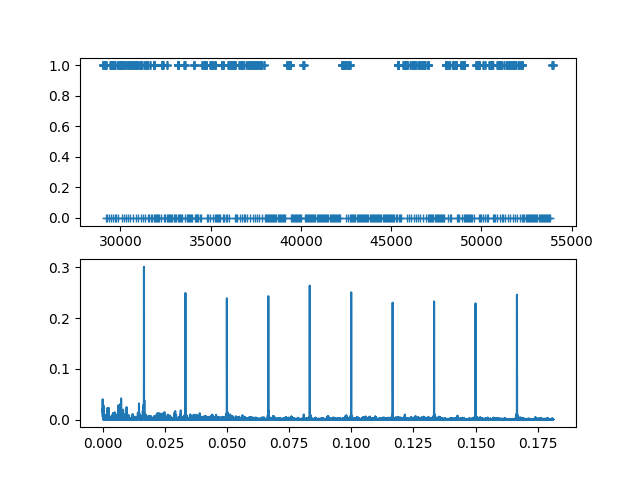
\includegraphics[width=8cm]{images/20201214_修士論文予稿/e70_c2.png}
  \caption{\ast\ast\ast.106.20.192の通信回数と解析結果}
  \label{fig:e70_result}
\end{figure}

また,ステータスコードに関してはC\&CサーバとTCPコネクションを確立できなったため取得できなかった.

\subsection{Case e435}
Case e435はCase e70と同様にマルウェア検体は動作したがC\&CサーバとTCPコネクションを確立できなかった事例で,e435のマルウェア検体のC\&CサーバのIPアドレスは\ast\ast\ast.24.93.253である.

表\ref{tab:e435_ip}はマルウェア検体が99.9\%の確率で周期的な通信を行った通信先のIPアドレス一覧である.表から2016年3月の28日から30日の3日間でC\&CサーバのIPアドレスを検出できた.
\begin{table}[htbp]
  \centering
  \caption{e435で周期的な通信を示した受信先IPアドレス}
  \begin{tabular}{|c||c|l|}
      \hline
      DATE & PERIODIC & IP ADDRESS \\
      \hline \hline
      2016/03/28 & 99.9\% & \begin{tabular}{l}
                            \textbf{\ast\ast\ast.24.93.253} \\
                            \ast\ast\ast.213.168.10         \\
                          \end{tabular} \\ \hline
      2016/03/29 & 99.9\% & \begin{tabular}{l}
                            \textbf{\ast\ast\ast.24.93.253} \\
                          \end{tabular} \\ \hline
      2016/03/30 & 99.9\% & \begin{tabular}{l}
                            \textbf{\ast\ast\ast.24.93.253} \\
                          \end{tabular} \\ \hline
  \end{tabular}
  \label{tab:e435_ip}
\end{table}

図\ref{fig:e435_result}は2016年3月28日にe435のマルウェア検体とC\&Cサーバと通信した回数と時間の関係を表した図である.図からマルウェア検体とC\&Cサーバは13分間に合計2578回通信していて,解析結果のグラフからピークは0.5868490564334333であることが分かる.この通信が99.9\%周期的であるために必要な値は0.011643320413840794で,ピークはこの値を超えているためマルウェア検体とC\&Cサーバ間の通信は周期的であると言える.
\begin{figure}[htbp]
  \centering
  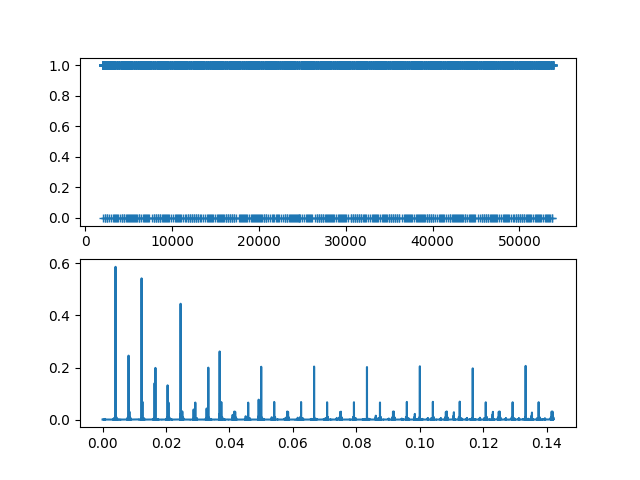
\includegraphics[width=8cm]{images/20201214_修士論文予稿/e435_c2.png}
  \caption{\ast\ast\ast.24.93.253の通信回数と解析結果}
  \label{fig:e435_result}
\end{figure}

また,Case e70と同様にCase e435でもC\&CサーバとTCPコネクションを確立できなかったためステータスコードを取得することができなかった.

\section{考察}
本章では実験結果からそれぞれの事例の通信の特徴とマルウェア検体の対処優先度について考察を行う.

データセットBOS\_2016の4つの事例(e12,e20,e70,e435)のうち,Lomb-Scargleピリオドグラムによってマルウェア検体とC\&Cサーバ間の周期的な通信を検出できた事例はe12とe70,e435の3事例のみであった.

そのうちC\&CサーバとTCPコネクションを確立できたe12のマルウェア検体は2つのC\&Cサーバと通信を行っていた.マルウェア検体と1つ目のC\&Cサーバ\ast\ast\ast.56.81.119の通信は5分間に複数回通信を行い,通信が発生しない時間が5分続いたあとにもう一度5分間通信して,その5分後に1回通信が発生した.さらに,その一連の流れを30分程度あとに再度繰り返していた.2つ目のC\&Cサーバである\ast\ast\ast.76.86.155との通信は1つ目のC\&Cサーバの186回と比べて40回しか発生していないが,複数回通信が発生し10分後に再度通信したあとに,40分程度通信が発生しない時間が続き同じような通信を行う,というように1つ目のC\&Cサーバと類似した通信の特徴を示した.これはC\&Cサーバから通信エラーを表すステータスコード403(Forbidden)が返ってきているため,マルウェア検体が何度もC\&Cサーバと正常に通信を試みようとしたことが原因であると考えられる.e12の通信観測データをLomb-Scargleピリオドグラムで解析した結果,周期的な通信を行っていた2つのC\&CサーバのIPアドレスを検出することができ,ステータスコードも取得できた.ステータスコードに関してマルウェア検体がC\&Cサーバ\ast\ast\ast.56.81.119と正常に通信できた回数が4回で,403(Forbidden)によって通信できなかった回数が16回であった.ステータスコード200(OK)が返ってきているが403(Forbidden)のほうが多く返ってきているのでこのC\&Cサーバに対する対処の優先度は低くすることができると考えられる.一方でマルウェア検体がC\&Cサーバ\ast\ast\ast.76.86.155と正常に通信できた回数が4回で403(Forbidden)によって通信できなかった回数が3回で正常に通信できた回数のほうが多くなった.そのため,1つ目のC\&Cサーバ\ast\ast\ast.56.81.119よりも対処の優先度を高くする必要があるといえる.

e12とは違い,e70やe435はマルウェア検体がC\&Cサーバに対してSYNパケットを送信したがサーバの応答がなかったため,TCPコネクションを確立できなかった事例である.こういった事例の通信には,TCPコネクションを確立するためにマルウェア検体が何度も短い間隔でC\&CサーバにSYNパケットを送信するという特徴がある.Lomb-Scargleピリオドグラムでe70とe435の通信観測データを解析するとそれぞれのC\&Cサーバの周期的な通信を検出できたが,TCPコネクションを確立できていないためステータスコードを取得することができなかった.こういった事例はC\&Cサーバから攻撃命令などを受けないため対処の優先度は低くすることができる.

しかし,e20はe12と同様にC\&CサーバとTCPコネクションを確立できたがエラーなどによりC\&Cサーバと正常に通信できなかった事例だが,Lomb-Scargleピリオドグラムでの解析ではマルウェア検体とC\&Cサーバ間の通信を検出できなかった.これは1秒にも満たない短時間で少ない回数しか通信が発生しなかったことが原因と考えられる.そのため,C\&Cサーバから返ってきたステータスコードも取得できないのでこのマルウェア検体の対処優先度を決定することはできなかった.

\section{おわりに}
本研究はネットワークの通信をLomb-Scargleピリオドグラムによって周期性を検出することでボットネットとC\&Cサーバ間の通信を検出することと,C\&Cサーバのレスポンスによってボットネットの対処優先度を決定する手法を提案する.

実験ではデータセットBOS\_2016のうち,C\&CサーバとTCPコネクションを確立できたがマルウェア検体またはC\&Cサーバ側のエラーによって通信が成立しなかった2つの事例(Case e12,e20)と,C\&CサーバとTCPコネクションを確立できずにマルウェア検体がTCP SYNパケットを送信し続けた2つの事例(Case e70,e435)の通信観測データを用いて実験を行った.実験の結果,4事例のうちe12とe70,e435の3つの事例でLomb-Scargleピリオドグラムによってマルウェア検体とC\&Cサーバの周期的な通信を検出することができた.また,C\&Cサーバとコネクションを確立できたe12でC\&CサーバからのHTTTPレスポンスのステータスコードを通信観測データから取得することができ,そのステータスコードから対処の優先度を決定することができた.コネクションを確立できなかったe70やe435のような事例であってもC\&Cサーバとの通信を検出できたため対処するべきであると判断できた.一方でe20のように短時間に少数の通信しか発生しなかった事例に関しては,Lomb-Scargleピリオドグラムによる周波数解析ではマルウェア検体とC\&Cサーバ間の周期的な通信を検出することができなかった.そのため,C\&Cサーバからのレスポンスも検出できないのでステータスコードに基づいた対処優先度を判断できなかった.

ボットウイルスを含めマルウェアに感染していないデバイスでも,Windowsアップデートやソフトウェアのアップデート,定期的に実行されるプログラムによって発生する通常の通信には周期性がある.Lomb-Scargleピリオドグラムによる解析ではそれらの通信を周期的な通信と判断してしまうが,そういった通信はマルウェアによる周期的な通信よりも通信間隔が長いことが多いため解析を行う通信観測データの時間範囲を狭くすることで検出を回避できると考えられる.また,通信先が安全だと分かっているIPアドレスのリスト(アローリスト)を定義することでも同様に検出を回避できる.

\bibliographystyle{junsrt}
\bibliography{DB}
\end{document}